%SETTINGS{{{
\documentclass[11pt]{iopart}
\usepackage{graphicx}
\usepackage{iopams}

% Fixing iopams poor centering of equations:
\expandafter\let\csname equation*\endcsname\relax
\expandafter\let\csname endequation*\endcsname\relax
\usepackage{amsmath}
%
%}}}
\begin{document}
%TITLE_ABS{{{
\title[]{FYP}

\author{Donovan Webb}

\address{Department of Physics,
University of Bath, Bath BA2 7AY, United Kingdom}
\ead{dw711@bath.ac.uk}

\begin{abstract}

XXPREVIOUSXX
A device capable of uniformly concentrating a magnetic fields inside of
a free space cavity will increase the efficiency of many magnetic
devices and sensors.  This project shall look at a proposed design for
a magnetic field concentrator informed by the transformation optic
technique. A metamaterial shell comprised of high and low permeability
sections alternating in the angular direction has been shown to
approximate the designed concentrator\cite{N2014}. The ability of the shell acting
as a concentrator will be explored in various regimes with a specific
focus on improving efficiency of wireless power transmission.

\end{abstract}
%}}}
%INTRO{{{
\section{Introduction}
%% - Motivation and overview brief description of power transfer problem

The manipulation of magnetic fields is a critical tool for many modern
technologies. Magnetic devices often have efficiencies dependent on
the strength of interaction with an external magnetic field. Examples
include energy harvesting from magnetic fields~\cite{HARVESTING} to
brain activity scans by locating small magnetic
gradients~\cite{BRAIN}. These devices may have increased efficiency by
concentrating the desired magnetic field within the area of sensing or
harvesting. \\ Magnetic fields may be described by Maxwell's
equations~\cite{MAXWELL} and are guided by materials due to their
optical properties, such as permitivity and permeability~\cite{OPTICAL
  PROPERITES}. Fermat's principle of least time allowed the design
of many optical devices using geometrical lenses~\cite{FERMAT},
however, with the maturation of fabrication techniques, many materials
may be produced with exotic anisotropic optical properties~\cite{META}
prompting the development of transformation optics (TO) --- a modern
approach to optical device design.\\ Here we describe one such TO
designed device; The magnetic concentrator~\cite{PRATT}, with a particular focus
on its efficacy in wireless power transmission. \\ 

\begin{figure}
  \begin{center}
   \noindent\includegraphics[width=0.75\linewidth]{images/trans_Opt_edit.pdf}
  \label{fig:TO}
  \end{center}
  \caption{The steps of Transformation Optics. a) A ray (red)
    travelling in untransformed spatial coordinates (black grid)
    follows the path of least time. b) A spatial coordinate
    transformation $A$ is applied to guide the ray along a desired
    path. c) A material (blue) is insterted into the untransformed
    space with corresponding permeability and permitivity which mimics
    the spatial coordinate transform $A$ for the ray. }
\end{figure}

\subsection{Transformation Optics and Metamaterials}
TO informed the design of many new devices such as perfect
lenses~\cite{}, magenetic-hoses~\cite{}, -cloaks~\cite{},
-rotators~\cite{}, -blackholes~\cite{}, and -concentrators~\cite{}. It
can be shown that due to the form invariance of Maxwell's equations, a
spatial coordinate transform is equivalent to the insertion of a
material with specific permeabilities and permitivities. This is shown
conceptually by the three steps of the schematic shown in
figure~\ref{fig:TO}. First a ray is considered in free cartesian space
in panel $a$, which due to Fermat's principle of least time will be
following the horizontal spatial grid lines.  The space is then
transformed arbitrarily in panel $b$ so that the ray adopts the
desired path for the final device. The transformation required, $A$,
to morph the ray now informs the optical properties for the specific
inserted material of panel $c$, which is once again located in
untransformed space.\\ The form invariance of Faraday's law is
described by the equivalent expressions

\begin{equation}
  \label{ME1}
  \nabla'\times \textbf{E'} = -jw[\mu_0]\textbf{H'}
  ~~~~~~~~and~~~~~~~~
  \nabla\times \textbf{E} = -jw[\mu']\textbf{H},
\end{equation}

where the first is expressed in transformed coordinate space $x'(x, y,
z), y'(x, y, z), z'(x, y, z)$ and free space permeability $[\mu_0]$,
whilst the second is expressed in untransformed cartesian space $x, y,
z$ but with some space dependent permeability $[\mu']$. Similar
equivalent expressions exist for the other Maxwell equations but with
some non-free permittivity $[\epsilon']$.\\
The required permeability and permittivity is found by,

\begin{equation}
  \label{eqn:J}
  \mu'=\frac{A\mu_0 A^T}{|A|}
  ~~~~~~~~and~~~~~~~~
  \epsilon'=\frac{A\epsilon_0 A^T}{|A|}
\end{equation}

where $A$ is the Jacobian matrix describing the transformation of
coordinate systems (e.g. between panel $a$ and panel $b$ in
figure~\ref{fig:TO}). \\
The resulting calculated optical properties may be anisotropic, have
arbitrary magnitude and even be negative~\cite{}. As bulk materials rarely, if
ever, show these properties, optical metamaterials are often
required~\cite{META3}. \\
Metamaterials are often comprised of repeating units whose dimensions
are much smaller than the wavelength of the interacting
radiation~\cite{META2}. The individual units may have specific
geometery, orientation and optical properties to selectively interact
with incident waves so that the net effect of the material mimics a bulk
substance with different optical properties than its substituent
parts.\\

\subsection{Magnetic Concentrator}
As described above, a device capable of magnetic field concentration
can increase the efficiency of sensors and energy harvesters.
Utilising TO we may design an optimal field concentrator which fulfils
the criteria: All magnetic field within a region $A$ is confined to
region $B$ where $B$ is free space only. A possible geometry for this
device that has cylindrical symmetry is shown in
XfXfigure~\ref{fig:shell}. A ray diagram
is shown in XfXfigure~\ref{fig:shell_TO} for free space with no
inserted material. Two coordinate transforms are now applied: First
the region $\rho < R_2 - \eta$ is radially and linearly compressed to
the region $\rho < R_1$; Second, to ensure the continuity of our
transformed space, a high ($k^{th}$) order polynomial radial expansion
of $R_2 - \eta < \rho < R_2$ to the region $R_1 < \rho < R_2$ is
made. These transformations are described by the coordinate
transformations,

\begin{equation}
  \label{transform}
\rho' = \frac{R_1}{R_2-\xi}\rho,~~~~~~~~\rho'\in[0,~R_2-\xi)~~\\
\rho' = R_2^{1-k}\rho^k.~~~~~~~~~\rho'\in[R_2-\xi,~R_2)
\end{equation}

By symmetry we see that $\theta$ and $z$ remain unchanged through the
two transformations. The corresponding Jacobians may be found for
these transformations and using equation~\ref{eqn:J}, the
permeabilities of the required inserted material may be found to be

\begin{equation}
  \label{eqn:mat}
  \begin{split}
 \mu' = \begin{pmatrix}1&0&0\\0&1&0\\0&0&(\frac{R_2-\xi}{R_1})^2\end{pmatrix}~~~~~~~~~~~~~\rho'\in[0,~R_1)~~\\
~~~~~~\mu' = \begin{pmatrix}k&0&0\\0&1/k&0\\0&0&\frac{1}{k}(\frac{\rho'}{R_2})^{2/k-2}\end{pmatrix}~~~~~\rho'\in[R_1,~R_2)
  \end{split}
\end{equation}

Taking the limit $\eta \rightarrow 0$ in order to concentrate all of
the field within $A$ into $B$, and matching the boundary conditions at
$R_2-\eta$ and at $R1$, we find that $k \rightarrow \infty$. From this
we find that the required permeability within $B$ is satisfied by free
space whilst a material with radial permeability $\mu_\rho \rightarrow
\infty$ and angular permeability $\mu_\theta \rightarrow 0$ is
required for region $A$. The $z$ components of permeability is ignored
as we assume it to be invariant if the cyclindrical shell is
significantly extended in the $z$ direction.\\
To satisfy this highly anisotropic condition, an exploration of
metamaterials is required. A possible discretized shell construction
is proposed~\cite{PRATT} where the high radial permeability is
provided by ferromagnetic materials whilst the angular permeability is
shielded by superconducting material. Materials such as MuMetal, have
relative permeabilities of up to XvX~\cite{MUMETAL} and ideal
superconductors in their Meissner state will exclude all magenetic
fields from within their interior giving a relative permeability of
$0$~\cite{Meissner}.  These two materials may be arranged in
alternating angular sheets, as seen in figure~\ref{fig:shell}, to
approximate the conditions proposed by TO design. \\
XeX discuss where this concentration originates? \\
In an external static uniform magnetic field, the ideal shell will
increase the field within region $B$ by a factor of
$R_2/R_1$. Similarly if a dipole with magnetic moment $m$ is present
at the origin and surrounded by the magnetic concentrator shell, then
the field outside of the shell will be increased by a factor of
$R_2/R_1$. Therefore for an observer at $\rho > R_2$ it will appear
that a dipole with magnetic moment $m\cdot R_2/R_1$ is present at the
origin.\\

(Comparison to other conc. techniques:
It is known that ferromagnetic materials concentrate magnetic fields
within their bulk~\cite{ferro} however, concentration of the field
into a free space cavity may be required.)

\begin{figure}
  \begin{center}
   \noindent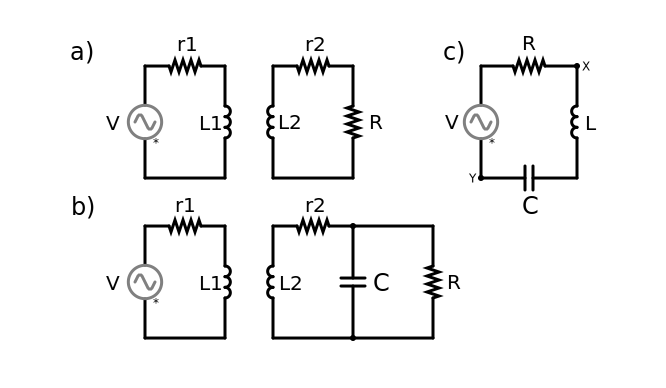
\includegraphics[width=0.75\linewidth]{images/WPT.pdf}
  \label{fig:WPT}
  \end{center}
  \caption{Wireless power transmission by inductive coupling. a)
    Simple circuitary for coupling $L1$ and $L2$ coils. The useful
    power transmitted is across load resistance $R$ whilst power lost
    is internal resistance of coils, $r1$ and $r2$. b) The receiving
    inductor is now part of a resonant RLC circuit. c) A series RLC
    circuit --- when voltage at $x$ and $y$ are in phase, the resonant
    condition is met.}
\end{figure}

\subsection{Wireless Power Transfer}
The ability to transfer power between devices that are not connected
by wires is useful in many settings: for convenince, e.g. mobile
phones; for safety, e.g. implanted medical devices; or for
practicallity, e.g. satellites.\\ We shall focus on near field power
transmission by the use of inductive coupling. Inductive coupling
transfers power between two coils of wire by an oscillating magnetic
field as seen in figure~\ref{fig:WPT}~$a$. The transmitting coil is
supplied with an alternating current, which by Ampere's law creates an
oscillating magnetic field. The receiving coil is placed within this
magnetic field, so that a current is induced as described by Faraday's
law.\\ This strategy for power transfer is highly sensitive to
distance as the magnetic field of a dipole drops off with distance
cubed.  The overall efficiency therefore suffers with distance as the
non-ideal resistive losses in the primary coil remain constant with
distance. To somewhat counteract this sharp drop off of efficinency
with distance, concentrating shells may be used to magnify the
transmitted field and locally concentrate the field around the
receiving solenoid. \\

%% - Wireless power transfer - lit review
%% - Where this work fits in overall field
%%%--------------------------------------------------------------------

%}}}
%METHODS{{{ 
\section{Methods}
\subsection{Construction of shell}
$0.X$~mm MuMetal XXX and $0.X$~mm copper was cut into $X$ by $X$ rectangular sheets. 
A plastic support for holding the MuMetal and Copper sheets was 3D printed using an ultimaker XX to produce the shells seen in figure~\ref{fig:shells}, with an $R_2/R_1$ ratio of XXX.\\

\subsection{DC Magnetic Fields}
Helmholtz coils were powered by a constant DC current to create a
uniform magnetic field within their center. A commercially available
XXX Hall probe was zeroed by using a MuMetal cannister, and then
placed at the center of the Helmholtz coils.  A Hall probe relates a
measured Hall voltage, $V_H$, to a surrounding magnetic field, $B$
\cite{XXX} as
\begin{equation}
  V_H = \frac{IB}{net}.
\end{equation}
The probe maintains constant current supply $I$, and material
paramaters $n$ (charge carrier density), $e$ (charge of electron) and
$t$ (thickness of probe) meaning a calibrated probe may give accurate
readings for magnetic fields.\\
The magnetic field, $B$, produced at the center of Helmholtz coils
with radius $R$, seperated by a distance $R$ should follow,
\begin{equation}
  B = \frac{8}{5\sqrt{5}}\frac{\mu_0 nI}{R},
  \label{eqn:helm}
\end{equation}
where $I$ is the current supplied to the coils and $n$ is the number of
turns of wire. This equation follows directly from the Biot-Savart law
\cite{XXX} and the relative geometry of the coils as seen in
figure~\ref{fig:helm}. From equation~\ref{eqn:helm} it can be seen that
the magnetic field should increase linearly with supplied
current. Using the Hall probe we ensured this was the case and found
the relationship of current supplied to magnetic field produced for
our paticular Helmholtz arrangement.\\ Now, with the capability to
produce known external magnetic fields, the described field
concentrating shells may be placed within this field and the Hall
probe may be placed within their inner radius to measure concentrated
field.

\subsection{AC characterization}
Initially the Helmholtz arrangement was repeated for exploration of
the concentrating shells behaviour in alternating magnetic
fields. However, instead of a Hall probe, a small solenoid was used to
detect the oscillating field. From Faraday's law, a voltage will be
induced in a wire loop due to a time dependent magnetic field. A
series of loops constituting a small solenoid will respond to a
sinuisoidal magnetic field, $B = B_0\cos{wt}$, with the relationship,
\begin{equation}
  V = -NAB_0\omega\sin{\omega t},
  \label{eqn:far}
\end{equation}
where $A$ is the area of one loop and $N$ is the number of loops,
$\omega$ is the angular frequency of the alternating magnetic field
and $t$ is time.\\ As $\omega$ is known and all other parameters
except external field are kept constant, the voltage across the
solenoid may be measured experimentally to find the relative magnetic
field strength.\\
The solenoid must however be characterized in order to find the
absolute magnetic field values. This was done by measurement of the
self inductance, $L$, of the solenoid as, XXX
\begin{equation}
  L = \mu_0\mu_rN^2A/l
\end{equation}
XXX

Due to the induced voltage across the inductor being small and
background noise being high, a lock-in amplifier was used to select
only the desired signal frequency. This substantially reduced noise in
our readings allowing higher frequency and lower magnetic field
strength experiments.\\
Use of solenoid, limitations of Helmholtz and pick up.

\subsection{Power Transfer}
Use of RLC circuitary.\\
Power transfer experiments measure power dropped across a load
resistor in a receiving circuit verses power lost in the transmitting
circuit's inductor. The receiving circuit, seen in
figure~\ref{fig:WPT}~$a$, has multiple arrangements to optimise
power transfer. The simplest of which is the load resistor in series
with the receiving inductor. In this case the optimal load resistance
is $R = \omega*L$, where $\omega$ is the angular frequency of the
oscillating magnetic field and $L$ is the circuit inductance.\\ To
maximise power transfer an RLC circuit is constructed on the receiving
circuit. Ideally in an RLC circuit the complex impedance of the
inductance and capacitance cancel leaving only the load
resistance. Our inductance is set by the solenoid we chose to use and
so for exploring power transfer at various frequencies, a capacitance
can be found to satisfy the resonance condition. If inductance, $L$,
does not vary then capacitance, $C$, is easily found by,
\begin{equation}
  C = \frac{1}{w^2L}.
\end{equation}
However, we need not assume that inductance is constant. A series RLC
circuit can be constructed as seen in figure~\ref{fig:WPT}~$c$ to
ensure resonance is met. Resonance occurs in this circuit when $V_x$
is exactly in phase with $V_y$. In this case any imaginary impedances
are cancelled and only real resistance remains. \\ For maximal power
transfer a parallel RLC circuit is preferable however due to the
restraints of the experiement a non-ideal version must be made as seen
in figure~\ref{fig:WPT}~$b$. The resonant condition found by the
series RLC is a close approximation to this more complicated parallel
circuit. \\
To maximise power transfer in the series RLC case, a familiar idea of
impedance matching occurs, i.e. Power is maximised when the load
resistance is equal to any internal resistances of the
components~\cite{XXX}. As internal resistances are difficult to
measure and may depend on current XXX, this could also be found
experimentally by measuring voltage and current over the load
resistance whilst varying load resistance. \\ For the parallel RLC
case, a more complicated expression for optimal load resistance was
found which depends non trivially on a combination of internal
resistances. A model is proposed below, however, experimentally
locating the optimal resistances was chosen as measuring internal
resistances proved difficult and time consuming.\\
XXTheory of Rload dependence on power transfer. \\


%% - Do not gloss over too many details
%% - Do discuss calibration of devices
%% - Circuitary for both DC, AC and power transfer.
%% - RLC parallel tuning
%}}}
%RESULTS{{{
\section{Results}
%% - Key results only!
%% - Discuss observed trends
%%     - Concentration factor
%%     - Power transfer
%% - Discuss sources and magnitude of errors
%% - Simulations
\subsection{DC Magnetic Fields}

\begin{figure}
  \begin{center}
   \noindent\includegraphics[width=0.75\linewidth]{images/DC-graph.pdf}
  \label{fig:DC_graph}
  \end{center}
  \caption{How concentration factor depends on frequency for a shell concentrating a static external field into its interior.}
\end{figure}

Using the DC Helmholtz set up as described in Methods, we observed
constant concentration factors for different shell constructions in an
external magnetic field ranging from $1$~G to $22$~G. No shell, 18
MuMetal, 36 MuMetal, 18 Copper and 18 MuMetal + 18 Copper shells were
used and their concentration factor with field may be seen in
figure~\ref{fig:DC_graph}, where concentration factor is defined as
(Internal Field)/(External Field). \\ It was found that the shell
contruction of 36 MuMetal thin sheets gave the optimum concentration
factor of $C = 2.38$ with minimal error ($0.1\%$) at higher field
strengths and a maximum error of $4.0\%$ at an external field of
$1.4$~G. This increase in error at low magnetic fields is due to
limited sensitivity of our Hall probe and current measurements over
the Helmholtz coils.\\ Similar error relationships are observed for
the other constructions. It should be noted that we assume the dipole
has been placed in the same position and orientation in all
experiments and so errors due to placement are excluded here.\\ It is
expected that the copper will have no effect on a static magnetic
field and this was confirmed by the $18$ copper shell displaying no
concentration of internal field.  This is due to copper having a
relative permeability similar to air, $\mu_r = 1.0$, and so negligible
field guiding properties. In the oscillating magnetic field regime
copper is expected to shield angular fields due to the production of
eddy currents. Only air-gaps are used to block the angular component
of a static magnetic field within our shells to simplify the
experimental set up, however superconducting sheets in a similar shell
have been shown to improve the concentration of static
fields~\cite{PRATT}.\\

\subsection{AC characterization}

\begin{figure}
  \begin{center}
   \noindent\includegraphics[width=0.75\linewidth]{images/AC-Helm.pdf}
  \label{fig:AC_helm_graph}
  \end{center}
  \caption{How concentration factor depends on frequency for a shell
    concentrating an oscillating external field into its interior.}
\end{figure}

\subsection{Helmholtz}
The Helmholtz coils were supplied with an alternating current in order
to create an oscillating magnetic field.  As described in Methods
equation~\ref{eqn:far}, the voltage induced across a solenoid is used
to detect the alternating magnetic field strength. The concentration
factor for a range of frequencies using various shell arrangements was
again explored.\\
The concentration factors between $0.5$~kHz and $30$~kHz can be seen
in figure~\ref{fig:AC_helm_graph}. It was found that a mixed shell of
alternating $18$ copper and $18$ MuMetal sheets had the optimum
concentration factor of $C = 3.12$ XeX at $5$~kHz.\\ Here we can see
that the copper sheets have a concentrating effect dependent on
frequency.  We found that the copper shell increases in efficacy from
$C = 1.0$ at $50$~Hz to $C = 1.3$ (2SF) at $10$~kHz and does not
increase substantially more as frequency is increased.  This behaviour
is expected as copper will shield perpendicular alternating magnetic
fields by the generation of eddy currents. This effective increase in
$\mu_\theta$ is desired for the optimal TO concentrator. However, it
is suprising that this shielding gives a maximum effect at this low
frequency. The skin depth of copper at $10$~kHz is $0.66$~mm which is
greater than the $0.3$~mm thickness of copper used within the
shell.\\ Supporting work done on COMSOL, seen in
figure~\ref{fig:COMSOL_CU}, suggests a similar observed effect where
36 copper sheets increase rapidly in concentration factor from $C = 1$
at $0$~Hz to $C = 1.5$ (2SF) by $10$~kHz and then only a small further
increase in efficacy at high frequencies.\\
The strong linear decay of field concentration after $5-10$ kHz for
all configurations is a suprising result which, although may be partly
due to the MuMetal's permeability frequency response, also appears to
occur at too low a frequency.\\ The COMSOL simulations do not show
this relationship which suggests the source may be either not modelled
appropriately within COMSOL or be a fault in this experimental
design.\\ Apart from instrument and measurement reading errors which
constitute only a small error (XXX\%), we observed errors due to stray
magnetic fields inducing pick-up within cables connecting the solenoid
to the lock-in amplifier. This source of noise is highly frequency
dependent and is at the same frequency as our desired signal, so
cannot be removed by the use of a lock-in amplifier. To supress this
noise careful cable placement and shielding was installed however,
from figure~\ref{fig:Noise} it can be seen that as current was
reduced, the measured voltage was still non-zero.\\ XXX A correction
was attempted...\\
This source of error prompted a decision to focus on two dipole
coupling experiments as the field produced by a dipole has a strong
distance drop off meaning unwanted pick-up in cables can be greatly
reduced.\\

\subsection{Power transfer}

\begin{figure}
  \begin{center}
   \noindent\includegraphics[width=0.75\linewidth]{images/RL-R.pdf}
  \end{center}
  \caption{How power transfer efficiency depends on load resistance in
    a coupled inductive circuit for various
    frequencies. \label{fig:RL-R}}
\end{figure}

\begin{figure}
  \begin{center}
   \noindent\includegraphics[width=0.75\linewidth]{images/RL-F.pdf}
  \end{center}
  \caption{How power transfer efficiency depends on frequency in a
    coupled inductive circuit.}\label{fig:RL-F}
\end{figure}

First we show the simplest power transfer experiment where the load
resistance is in series with the receiving inductor -- an RL
circuit. Figure~\ref{fig:RL-R} shows the relative PTE versus load
resistance for various frequencies. The peaks of these curves confirm
the expected optimum load resistance of $R = \omega L$. \\ An
Oscillating magnetic field, $B$, produced from a solenoid and
concentrated by a shell follows,
$$B = CI\mu_0n\cos{\omega t},$$
where $C$ is the concentration factor, $I$ is the current through the
solenoid and $n$ is the number of turns of the solenoid.  If a second
solenoid is placed within the field of the first, as shown in
figure~\ref{fig:dipole-dipole}, then voltage will be induced across it
according to Faraday's law,
$$V = -NA\frac{dB}{dt},$$
$$V = C\omega I NA\mu_0n\sin{\omega t},$$
where $N$ is the number of turns of the solenoid and $A$ is the area
of one turn.
The power dropped across a resistor with magnitude $\omega L$ in
series with this inductor will then be described by,
$$ P = V^2/R $$
$$ P = \frac{C^2wI^2k}{L}\sin{\omega t}^2$$
where $k$ is the collection of constant coefficients that will remain
constant between different shells.  Max power received in the second
circuit is therefore proportional to $w \cdot \frac{C^2}{L} \cdot
I^2$. Plotting $\frac{P}{I^2}$ against angular frequency $w$ therefore
gives $\frac{C^2k}{L}$ as shown in XX figure~\ref{fig:RL-F}. Assuming
the coefficients in $k$ remain constant, comparisons of this gradient
between a concentrating shell with inductance $L_s$ and no shell with
inductance $L_0$ and $C_0 = 1$ yields,
\begin{equation}
  \eta = \frac{C^2L_0}{L_s},
  \label{eqn:eta}
\end{equation}
the effective concentration factor for power transfer. Figure
XXX~\ref{fig:RL-F} shows how $\eta$ depends on frequency for various
shell configurations.\\ As observed in the Helmholtz driven field
case, we see that the copper sheets increase in concentrating effect
rapidly between $0$ and $10$ kHz. The Copper only shell increases to
around $\eta = 2$ which, if it is assumed that $L_0 = L_s$,
corresponds to a power transfer increase of $2$x or a corresponding
field concentration of $\sqrt{2}$ within the shell's cavity. It can be
seen that using only MuMetal sheets gives a power transfer increase of
$6$x and a concentration of field that is independent of field
frequency for the range $0 - 30$ kHz. This differs from the previous
Helmholtz result where a steady drop off of concentration factor was
observed as frequency increased past $10$ kHz.\\ The mixed shell of 18
MuMetal sheets and 18 Copper sheets was found to have the best power
transfer increase of $9$x after the copper sheet effectively shields
the angular field at $10$ kHz. This power increase corresponds to a
magentic field concentration of $3$ within the shells
cavity.\\ Figure~\ref{fig:RL-F} XXX shows the optimal PTE for a range
of frequencies with different shell constructions around the receiving
inductor.  Assuming the inductance value remains constant with
different shell configurations (an exploration of this assumption is
considered in DiscussionXXX), absolute power transfer can be
calculated as described in Methods.  Table~\ref{table:RL_freq} gives
the maximal power transfer for different arrangements of shells.\\

\begin{figure}
  \begin{center}
   \noindent\includegraphics[width=0.75\linewidth]{images/RLC-P.pdf}
  \label{fig:RLC-P}
  \end{center}
  \caption{How the increase in power transfer efficiency depends on
    frequency in a coupled parallel RLC circuit.}
\end{figure}

Parallel RLC circuits are more fitting for optimising power
transfer~\cite{XXX}. For the arrangement described in
figure~\ref{fig:WPT}~$b$, a shell comprised of $18$ MuMetal and
$18$ Copper sheets was explored. The optimal load resistance was found
by taking voltage measurements across a range of load resistance. An
example power versus load resistance curve for $30$ kHz can be seen in
XXX figure~\ref{fig:parallel_R}.\\ Optimal load resistances were found
for a range of frequencies and PTE were calculated as shown in XXX
figure~\ref{fig:parallel_R}. Figure XX~\ref{fig:parallel_R} shows the
ratio of shell present versus no shell present for the range of
frequencies. It can be seen that the increase of ratio between $0$ and
$10$ Hz is still present, however due to the high error and few data
points, other trends are hard to distinguish. In this arrangement,
with the coils seperated by a distance of XXX mm, maximum observed
power transfer is XX $0.05\%$.\\
To further explore PTE, the distance between the two coils was
varied. With a distance of XXX mm and a full shell around the
receiving coil, a PTE of XXX\% was achieved.\\
It was expected that a shell around the transmitting coil would
further increase the field incident on the receiving coil. Therefore
the arrangement described in Methods Figure~\ref{fig:two_shell} was
constructed and the peak power transfer observed at $30510$ kHz was
found to be $1.01\%$.\\

% ------------------------------

\begin{figure}
  \begin{center}
   \noindent\includegraphics[width=0.75\linewidth]{images/temp-equiv_circ.png}
  \label{fig:RLC-eqcirc}
  \end{center}
  \caption{}
\end{figure}

\begin{figure}
  \begin{center}
   \noindent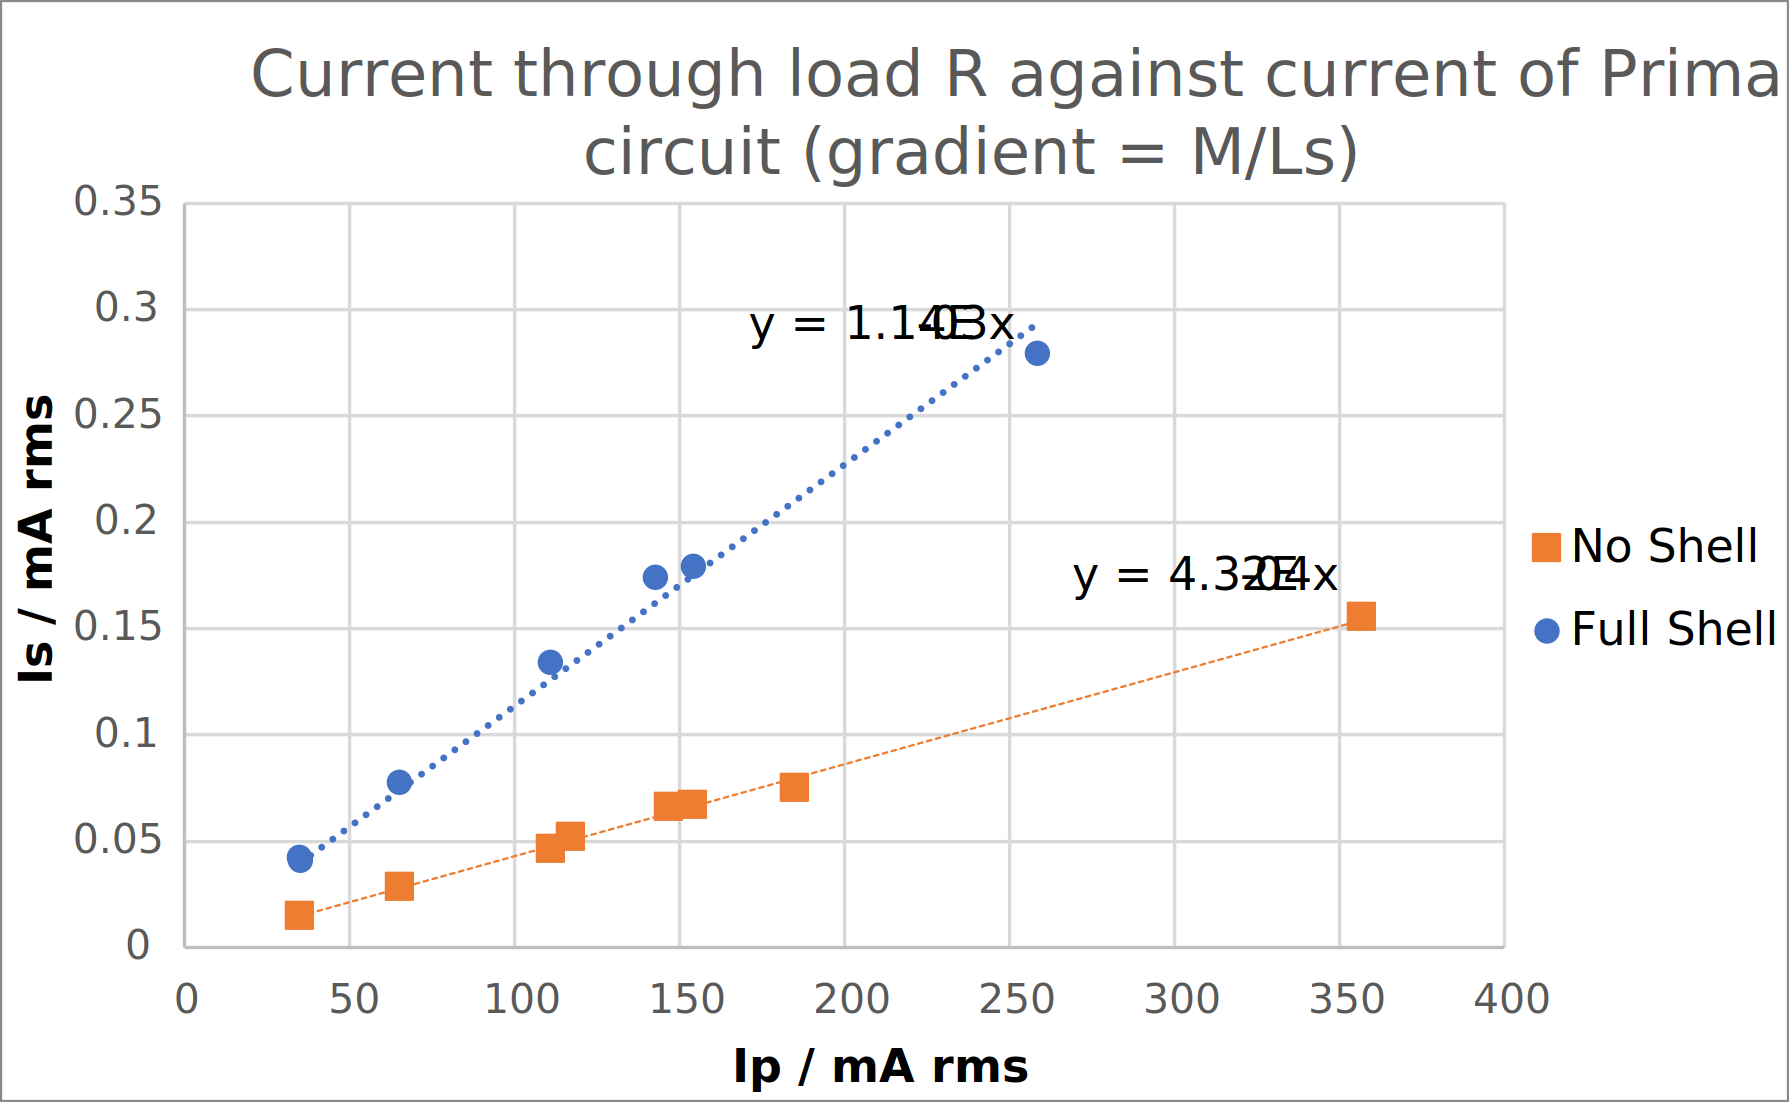
\includegraphics[width=0.75\linewidth]{images/Is_vs_Ip_RLC.pdf}
  \label{fig:RLC-IvI}
  \end{center}
  \caption{}
\end{figure}

\begin{figure}
  \begin{center}
   \noindent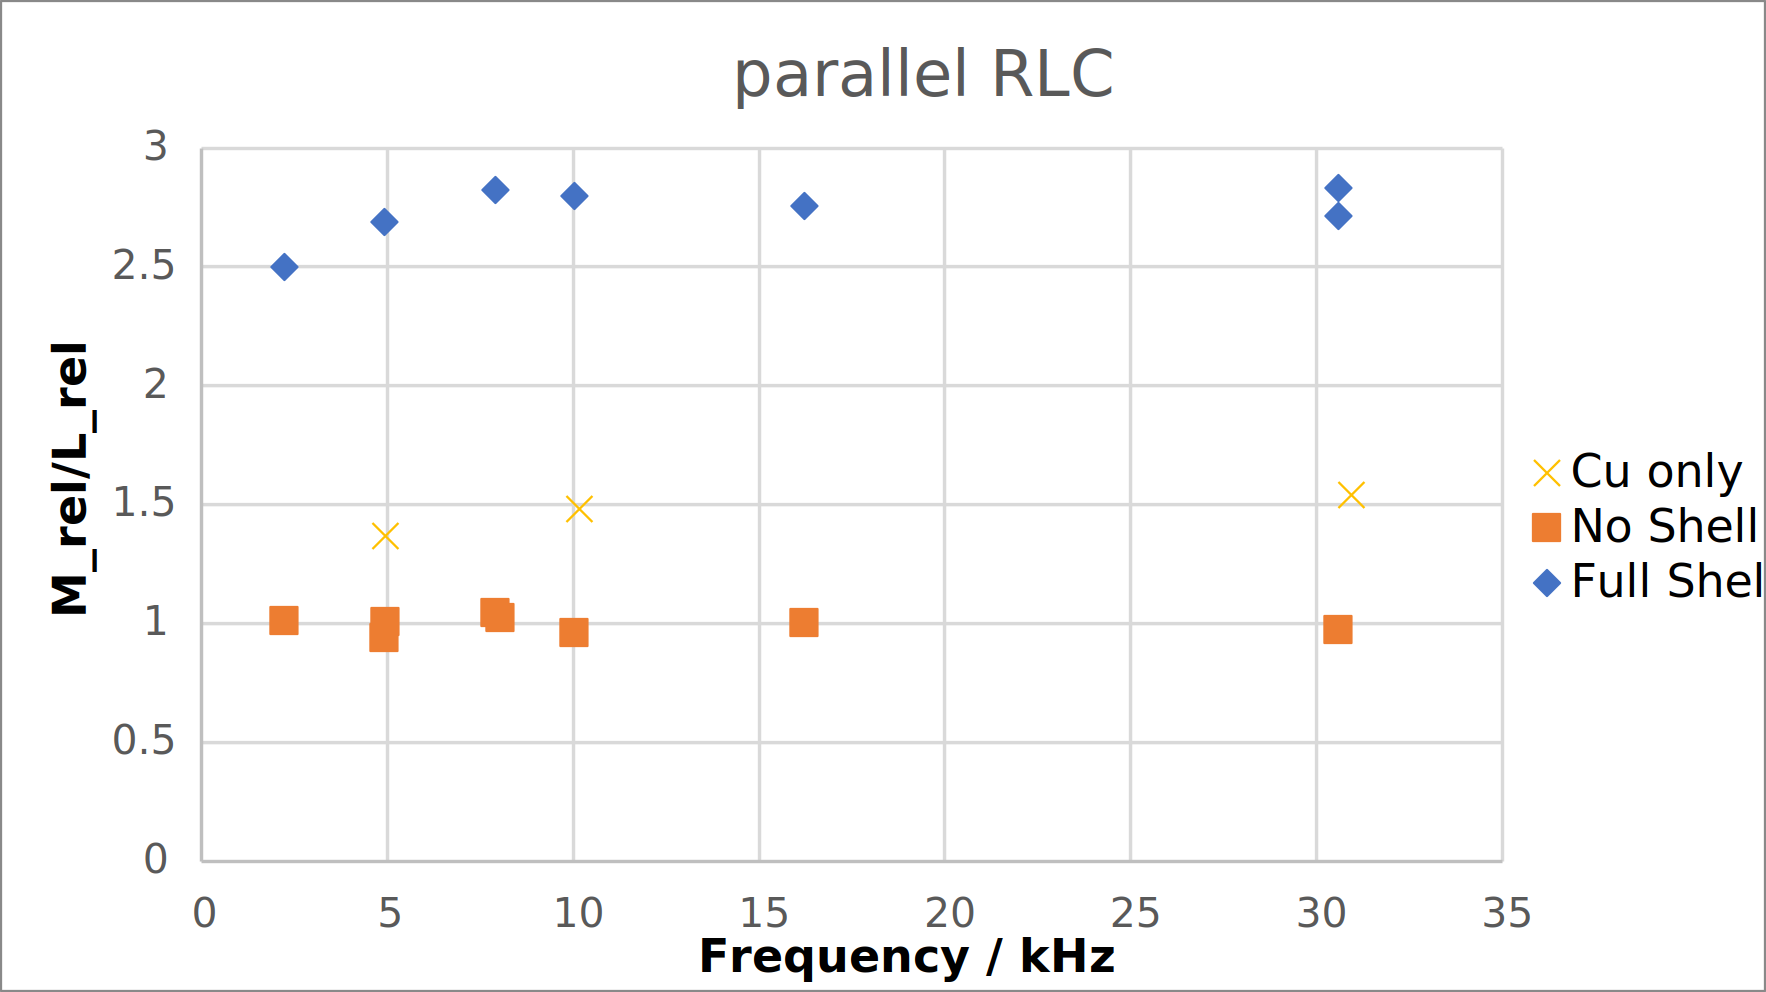
\includegraphics[width=0.75\linewidth]{images/parallel_RLC_Mrel.pdf}
  \label{fig:RLC-Mrel}
  \end{center}
  \caption{}
\end{figure}

Parallel RLC coupled to coil can be considered as
figure~\ref{fig:RLC-eqcirc}.  The voltage across $R_{load}$ is equal
to,
$$ V_s = j\omega MI_p - j\omega L_sI_s.$$
$I_s$ can be found by,
$$ I_s = j\omega MI_p / z_s $$
where $z_s$ is the total impedance of circuit 2...
$$ V_s = \frac{MR}{L_s}I_p. $$
Therefore a plot of $V_s / R$ against $I_p$ will yield a gradient of
$M/L_s$ as seen in figure~\ref{fig:RLC-IvI}.  Furthermore, $M =
M(\omega)$ for shells with copper present, and so a plot of
$(M/L_s)/(M^0/L_s^0)$ gives the relative increase in $M/L_s$ with
frequency as seen in figure~\ref{fig:RLC-Mrel}.\\


% INCLUDE? A summary of PTE and field concentration factors is shown in the table~\fig{table:summary}.\\

\subsection{Distance}
Experimentally we found that power drops off as $r^{-5.6}$ which is in
close agreement to the theoretical $r^{-6}$.\\

%}}}
%DISCUSSION{{{
\section{Discussion}
%% - Tee and Pi circuit analysis
%% - Models
%% - Overall trends matching simulation, analysis and Experimental
%% - Comparison with other published results
%% - Contextualize findings in light of other work

% Non ideal behaviour \\
For the constructed shells used in these experiments, their $R_2/R_1$
ratio was $40 \pm 2$ mm. From the theoretical TO work, it is predicted
that the field should be concentrated by the perfect shell by
$R_2/R_1$. We found a range of concentrations for both static, $C =
2.25 - 2.38$ XeX and oscillating, $C = 2 - 3.1$ XeX, external fields
whose maximum concentration factors are still well below the expected
theoretical concentration factor of $4.0 \pm 0.2$. This is likely
explained by our approach to approximating the perfect TO designed
anisotropic shells with shells comprised of discrete sections of high
and low permeability.  In both static and oscillating fields, we found
that 36 MuMetal sheets performed better than 18 MuMetal sheets which
suggests that finer discretization of the proposed shells gives
concentrations closer to the theoretical value. In the static field
experiments, only air was used to approximate the zero relative
angular permeability. Air has a permeability of $\mu = 1$, which
although is far less than the MuMetal's $\mu = XXX$, is likely still a
poor approximation. This can be seen by the increase in performance in
the oscillating external field experiments where copper sheets are
introduced in order to effectively screen out angular field density by
the production of Eddy currents. Eddy current screening is
proportional to frequency of the oscillating field~\cite{XXX}, and
therefore, it can be seen that the concentration factor for shells
with copper present increase with frequency. \\

Eddy currents may be modelled as a wire loop perpendicular to an
oscillating magenetic field. A current is produced within the loop
which is proportional to frequency of the field and, due to Lenz's
law, flows in a direction to oppose the change in field density. The
induced current in the loop is
$$ I = \frac{A}{R}\omega (B - B'), $$
and the field produced by the current is,
$$ B' = -I \mu_0 r. $$
Combining these equations give,
$$ B' = \frac{\omega B}{1+\omega}, $$
which may be seen plotted with the COMSOL and experimental results for
a copper only shell.\\

XwX Superconducting material has been suggested to effectively screen
angular field in the static case~\cite{XXX}... \\

% How L changes
\begin{figure}
  \begin{center}
   \noindent\includegraphics[width=0.75\linewidth]{images/inductance.pdf}
  \end{center}
  \caption{}\label{fig:inductance}
\end{figure}
For many results we have assumed that the inductance of the solenoid
was independent of the shell surrounding it. Here we shall reexplore
some results without this assumption. \\ The resonant condition of a
series RLC circuit,
\begin{equation}
  \label{eqn:RLC}
  \omega = 1/\sqrt{LC},
\end{equation}
allows the calculation of effective inductance $L$ using the known
capacitance, $C$ and measured frequency peak,
$\omega$. Figure~\ref{fig:inductance} shows $\omega^{-1}$ against
$\sqrt{C}$ to find inductance $L$. The observed inductances for the
two shell configurations are not sensitive to frequency however, it
should be noted that the inductance of the coils used does have a
dependency on current. For the range of currents used in the series
RLC experiment, this change in inductance with current was negligible
compared with the observed change in inductances with different
surrounding shells. It was found that the inductance when surrounded
by the full shell is $1.25\pm0.01$~mH whilst the bare solenoid and the
copper only shell give an inductance of $1.02\pm0.02$~mH. This
increase in inductance could be understood by the fact that the high
permeability MuMetal in the shell is located near to the coil,
increasing the relative permeability of space in the vicinity of the
coil. From equation~\ref{eqn:eta} it can be seen that the effective
power concentration, $\eta$, for the RL circuit is dependent on both
field concentration and effective inductance of the solenoid and in
fact the increase in effective inductance reduces the increase in
power transfer. The use of a tuned RLC setup within the receiving
circuit can counteract this loss of power concentration with increased
inductance as the load resistance no longer needs to match $\omega L$,
as discussed in Methods.\\

Due to the sharp drop off of power transfer with distance, the
greatest PTE found was $1.01\%$ XeX at a seperation of $48.7$~mm with
both the transmitting and receiving coil surrounded by a concentrating
shell. The reason for this poor efficiency is largely due to the
non-ideal real resistive component of the transmitting coil.

%%%%

DC:  \\
- further explanation on error source in placement \\

Linear decay of coil in non RLC \\
- Due to pick up that is proportional to $w^2$? \\
- Expected drop off due to magnetic saturation? or other reasons for
MuMetal failure. - COMSOL MU thickness \\

Power transfer \\
- Generally low PTE due to high loss of inductor.  Could have used
laminated AC inductor to reduce eddie currents.  Could have not used
iron core as hysteresis. \\
- Discussion of other power transfer techniques and coupled inductor
papers. Why a shell is better than no shell with distances. \\
- Why a shell allows a small radii inductor to be used - efficiency of scale
Better coupling for given distance. See p.51 pratt. \\
- Relationship of PTE with distance -$r^{-5.6}$. Effective mutual
inductance changed. \\
- Two shells present. \\
- Another exploration on error sources and summary of largest
sources.\\

Comparison of RL, series RLC and parallel RLC circuitary: \\
- models \\
- expected efficiency \\


can use a smaller solenoid, plot spider graphs in python\\
%}}}
%CONCLUSIONS{{{
\section{Conclusions}
EXTENSIONS \\
0) For further understanding we would need to look at more frequencies
and expecially at much higher freqs. A selection of different dipoles
would also be beneficial to ensure that frequency dependence is not
linked to non-ideal dipole.\\

0) Perhaps another circuit could be designed that works more similarly
to an RLC? Could propose one however experimentation has not been
performed.\\

0) Could a more complicated and directional shell be designed for
power transfer?\\
%}}}
%REF{{{
\section{References}
%}}}
\end{document}

